% --- Motivation: the memory wall ---
\begin{frame}{The Model Does Not Fit}
  \begin{itemize}\itemsep0.45em
    \item[\textcolor{red}{$\blacktriangleright$}] Take the smallest model anyone still calls a ``large'' language model: \textbf{7 billion parameters}. In \texttt{bf16} the weights alone are $7 \times 10^9 \times 2 = 14$\,GB, which fits comfortably on one GPU.
    \item[\textcolor{red}{$\blacktriangleright$}] \textbf{Training} it does not. Adam plus a mixed-precision master copy costs \textbf{16 bytes per parameter} of \emph{model state}, before a single activation is stored:
      \[
        7 \times 10^{9}\ \text{params} \times 16\ \frac{\text{bytes}}{\text{param}} = 1.12 \times 10^{11}\ \text{bytes} = \mathbf{112\ GB}.
      \]
    \item[\textcolor{red}{$\blacktriangleright$}] An NVIDIA H100 SXM has \textbf{80\,GB} of HBM3. An H200 has 141\,GB, a B200 has 192\,GB --- and the model people actually want to train is 70B or 405B, not 7B.
    \item[\textcolor{red}{$\blacktriangleright$}] So the first question of this lecture is not ``how do I go faster?'' It is \textbf{``how do I run at all?''} Speed is the second question.
  \end{itemize}
  \vspace{0.2em}
  {\scriptsize Throughout this deck $1\,\text{GB} = 10^{9}$ bytes. Card specifications: \href{https://www.nvidia.com/en-us/data-center/h100/}{NVIDIA H100}, \href{https://www.nvidia.com/en-us/data-center/h200/}{H200}.}
\end{frame}

\begin{frame}{Two Curves That Diverge}
  \begin{columns}[T,onlytextwidth]
    \column{0.53\textwidth}
      \begin{itemize}\footnotesize\itemsep0.45em
        \item[\textcolor{red}{$\blacktriangleright$}] \textbf{Model size} has grown by three orders of magnitude in six years; \textbf{GPU memory} per device by less than one. Rajbhandari et al.\ put the gap at ``over 1000$\times$'' against ``5$\times$''.
        \item[\textcolor{red}{$\blacktriangleright$}] The scaling laws from deck 07 say the loss keeps falling with parameters and tokens. Nothing in them says the result fits in one device.
        \item[\textcolor{red}{$\blacktriangleright$}] Two consequences follow:
          \begin{itemize}\itemsep0.2em
            \item Training state must be \textbf{split} across devices, not replicated.
            \item Whatever you split you must later \textbf{communicate} --- over links running at a quarter of HBM speed inside a node, and under a fiftieth of it between nodes.
          \end{itemize}
        \item[\textcolor{red}{$\blacktriangleright$}] Every technique here answers one question: \emph{which term do I shard, and what does the communication cost?}
      \end{itemize}
      \vspace{0.2em}
      {\scriptsize Growth figures: Rajbhandari et al., ``ZeRO-Infinity,'' \href{https://arxiv.org/abs/2104.07857v1}{arXiv:2104.07857v1}.}
    \column{0.45\textwidth}
      \centering
      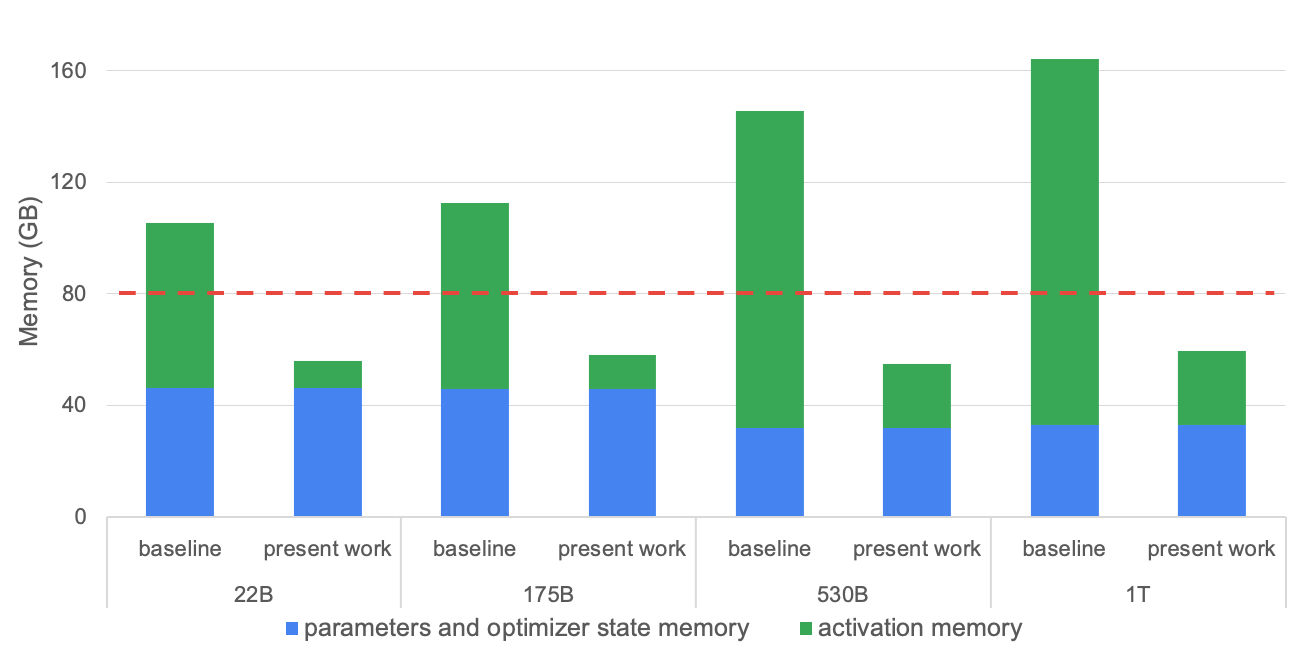
\includegraphics[width=\linewidth,height=0.62\textheight,keepaspectratio]{images/distributed-training/korthikanti_fig1_activation_memory_vs_a100.jpg}\\[0.3em]
      {\scriptsize Memory needed per GPU for four model sizes. The dashed red line is the 80\,GB capacity of an A100. Korthikanti et al., ``Reducing Activation Recomputation in Large Transformer Models,'' \href{https://arxiv.org/abs/2205.05198v1}{arXiv:2205.05198v1}, Figure 1.}
  \end{columns}
\end{frame}

\begin{frame}{Four Axes to Split On}
  \begin{itemize}\itemsep0.4em
    \item[\textcolor{red}{$\blacktriangleright$}] A training step is a four-dimensional object: a \textbf{batch} of examples, each of some \textbf{sequence length}, pushed through a stack of \textbf{layers}, each holding a \textbf{weight matrix}. You can cut along any of the four.
  \end{itemize}
  \vspace{0.3em}
  \centering
  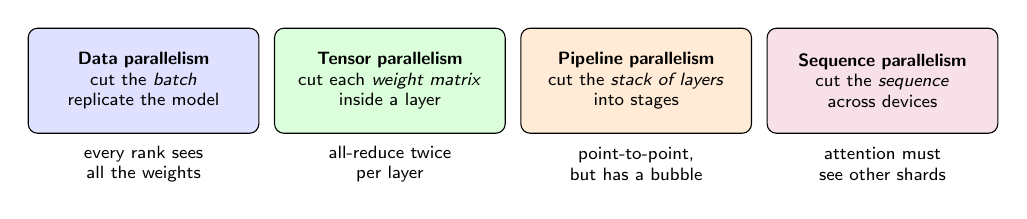
\begin{tikzpicture}[font=\sffamily\scriptsize, >=latex, scale=0.92,
      every node/.style={transform shape},
      ax/.style={draw, rounded corners=0.12cm, minimum width=3.15cm, minimum height=1.45cm,
                 align=center, text width=2.95cm, font=\sffamily\scriptsize}]
    \node[ax, fill=blue!12]   (dp) at (0,0)    {\textbf{Data parallelism}\\cut the \emph{batch}\\replicate the model};
    \node[ax, fill=green!14]  (tp) at (3.4,0)  {\textbf{Tensor parallelism}\\cut each \emph{weight matrix}\\inside a layer};
    \node[ax, fill=orange!16] (pp) at (6.8,0)  {\textbf{Pipeline parallelism}\\cut the \emph{stack of layers}\\into stages};
    \node[ax, fill=purple!12] (sp) at (10.2,0) {\textbf{Sequence parallelism}\\cut the \emph{sequence}\\across devices};
    \node[font=\sffamily\scriptsize, align=center] at (0,-1.15)    {every rank sees\\all the weights};
    \node[font=\sffamily\scriptsize, align=center] at (3.4,-1.15)  {all-reduce twice\\per layer};
    \node[font=\sffamily\scriptsize, align=center] at (6.8,-1.15)  {point-to-point,\\but has a bubble};
    \node[font=\sffamily\scriptsize, align=center] at (10.2,-1.15) {attention must\\see other shards};
  \end{tikzpicture}
  \vspace{0.4em}
  \begin{itemize}\footnotesize
    \item[\textcolor{red}{$\blacktriangleright$}] ZeRO and FSDP are a fifth idea layered on the first: keep data parallelism's simple programming model, but stop replicating the model state.
    \item[\textcolor{red}{$\blacktriangleright$}] Production pre-training runs use \textbf{three or four at once}. We build up to that combination in the pipeline-parallelism section.
  \end{itemize}
\end{frame}
